\section{Fundamentos de Internet y BGP} \label{sec:anexo_fundamentos_internet_bgp}


\subsection{Internet} \label{sec:anexo_internet}

Internet es una red global compuesta por múltiples redes interconectadas entre sí, que permite la comunicación y el intercambio de información entre dispositivos distribuidos geográficamente. 
Su funcionamiento depende de la cooperación entre distintos sistemas de comunicación, protocolos y organizaciones que administran diferentes segmentos de la red. 
Gracias a esta infraestructura, es posible ofrecer servicios como navegación web, correo electrónico, transmisión de contenido y múltiples aplicaciones distribuidas.\\


Desde una perspectiva estructural, Internet puede entenderse como una \textbf{red de redes}, donde distintos dominios administrativos se conectan para permitir conectividad global. 
Esta característica la convierte en un sistema distribuido de gran escala, dinámico y heterogéneo, en el cual la información puede viajar a través de múltiples caminos antes de 
alcanzar su destino final. Debido a esto una buen amanera de abstrar su funcionamiento y complejidad para su estudio es abstraer su estructura a una reprsenatcion en forma de grafo.\\


El correcto funcionamiento de Internet depende de la cooperación entre las diferentes partes que lo forma,es por esto que existe una jerarquia de organizaciones encargadas de coordinar los recursos y estándares. En particular, la \textbf{IANA} (\textit{Internet Assigned Numbers Authority}) 
administra globalmente recursos críticos como bloques de direcciones IP y números de Sistemas Autónomos. Estos recursos son luego distribuidos por los \textbf{Registros Regionales de Internet} 
(\textit{Regional Internet Registries}, \textbf{RIRs}), entre los que se encuentran \textbf{ARIN}, \textbf{RIPE NCC}, \textbf{APNIC}, \textbf{LACNIC} y \textbf{AFRINIC}, cada uno responsable 
de una región específica del mundo.
Asimismo, organizaciones como la \textbf{IETF} (\textit{Internet Engineering Task Force}) definen los estándares técnicos que permiten la interoperabilidad de Internet, incluyendo protocolos 
fundamentales como TCP/IP, DNS y BGP. Por su parte, la \textbf{ICANN} (\textit{Internet Corporation for Assigned Names and Numbers}) coordina el sistema global de nombres de dominio y participa 
en la administración de recursos de numeración a nivel internacional. Finalmente, los \textbf{Proveedores de Servicios de Internet} (\textit{Internet Service Providers}, \textbf{ISPs}) desempeñan 
un rol central al proporcionar conectividad a usuarios, empresas y otras redes, enlazando la operación de estas entidades con la infraestructura efectiva de Internet.\\


% \begin{figure}[H]
%     \centering
%     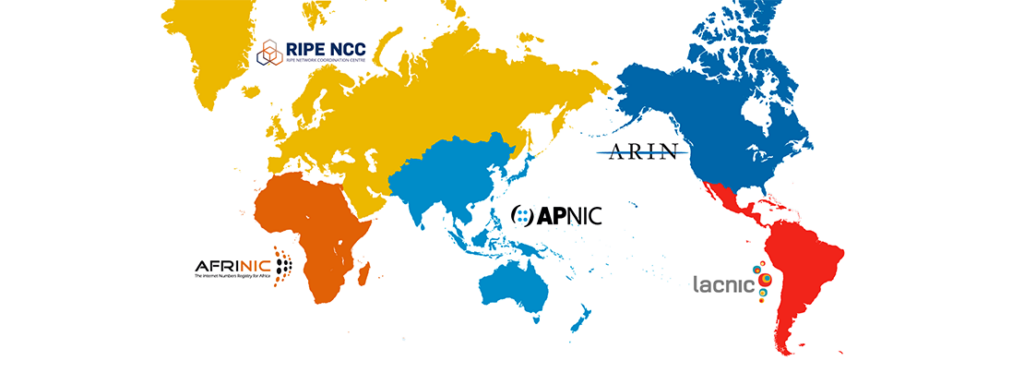
\includegraphics[width=0.6\textwidth]{Anexos/img/01/RIRs.png}
%     \caption{RIRs y su cobertura geográfica. Fuente: https://blog.apnic.net/2024/10/28/revising-the-criteria-for-the-accreditation-of-rirs/}
%     \label{fig:rirs_map}
% \end{figure}

\subsection{Sistemas Autónomos} \label{sec:anexo_sistemas_autonomos}


Como se habló previamente en la Sección~\ref{sec:sistemas_autonomos}, los \textbf{Sistemas Autónomos (AS)} son un conjunto de dispositivos que comparten un mismo protocolo de ruteo y son administrados por una misma entidad u organización, como proveedores de servicios de Internet (ISP), universidades, empresas o instituciones gubernamentales. 
La interconexión entre estos sistemas es la que da lugar a la estructura global de \textbf{Internet}.\\


Cada AS se identifica mediante un \textbf{Número de Sistema Autónomo} (\textit{Autonomous System Number}, \textbf{ASN}) que permite distinguirlo dentro del ecosistema de Internet. 
Además, cada AS administra o anuncia uno o más bloques de direcciones \textbf{IP}, los cuales son asignados por los \textbf{Registros Regionales de Internet} (\textit{Regional Internet Registries}, \textbf{RIRs}) , a partir de bloques delegados por la \textbf{Autoridad de Asignación de Números de Internet} (\textit{Internet Assigned Numbers Authority}, \textbf{IANA}).
En este proceso, los RIRs distribuyen recursos a los \textbf{Registros Locales de Internet} (\textit{Local Internet Registries}, \textbf{LIRs}), proveedores y usuarios finales.\\

Los ASNs pueden clasificarse en \textbf{públicos} o \textbf{privados}. 
Los \textbf{ASN públicos} son asignados por los RIRs y son únicos a nivel global, por lo que pueden aparecer en las tablas de enrutamiento públicas de Internet. 
En cambio, los \textbf{ASN privados} se utilizan en entornos internos, pruebas, simulaciones o conexiones cerradas entre routers, y no deben propagarse hacia la tabla global de Internet. 
Entre los rangos reservados para uso privado se encuentran 64512--65534 y 4200000000--4294967294 y estos estan indicados en el RFC 6996.\\ %TODO: citar

Desde el punto de vista de su rol dentro de la topología de Internet, los ASes suelen clasificarse en distintos niveles jerárquicos. 
Una clasificación ampliamente utilizada distingue entre \textbf{Tier-1}, \textbf{Tier-2} y \textbf{Tier-3}. 
Los ASes \textbf{Tier-1} corresponden a grandes proveedores globales de tránsito que conforman el \textit{backbone} de Internet y que intercambian tráfico entre sí sin pagar tránsito. 
Los \textbf{Tier-2} suelen corresponder a operadores regionales o nacionales que compran tránsito a redes Tier-1 y, a su vez, venden tránsito a redes de menor escala. 
Finalmente, los \textbf{Tier-3} suelen ser proveedores locales o redes de acceso que pagan por tránsito para ofrecer conectividad a usuarios finales~\cite{InterconnectionPeeringSettlements}.\\

Otra forma de caracterizar la posición de un AS dentro de Internet es mediante su \textit{customer cone}, es decir, el conjunto de ASes que puede alcanzar a través de relaciones proveedor--cliente. 
En este contexto, Luckie \textit{et al.}~\cite{ASRank} utilizan esta noción para estimar el grado de globalidad de un AS y su posición relativa en la jerarquía de Internet.
Si el \textit{customer cone} es mayor o igual a 200, se considera Tier-1, si es mayor a 2,000, se considera Tier-2 y si es menor a 200, se considera Tier-3.\\


Además de esta clasificación jerárquica, los Sistemas Autónomos pueden distinguirse según el número y tipo de conexiones externas que mantienen. 
En este contexto, un AS puede ser clasificado como:

\begin{itemize}
    \item \textbf{Stub AS}: se conecta únicamente a otro Sistema Autónomo y no transporta tráfico de tránsito para terceros.
    \item \textbf{Transit AS}: se conecta a múltiples Sistemas Autónomos y permite el tránsito de tráfico entre ellos.
    \item \textbf{Multihomed AS}: se conecta a más de un Sistema Autónomo para mejorar redundancia o disponibilidad, pero no ofrece tránsito entre ellos.
\end{itemize}

De manera relacionada, también es común distinguir entre ASes \textbf{\textit{single-homed}} y \textbf{\textit{multi-homed}}. 
Los primeros poseen una única conexión hacia otro AS, mientras que los segundos tienen conexiones hacia dos o más ASes. 
Esta distinción es importante, ya que influye en la resiliencia, redundancia y diversidad de rutas disponibles para una red.\\



En el contexto del enrutamiento interdominio también aparecen los conceptos de \textbf{\textit{upstream}} y \textbf{\textit{downstream}}. 
Un \textit{upstream} corresponde, en términos generales, al proveedor o red ubicada ``hacia arriba'' en la cadena de conectividad, es decir, 
aquella de la cual un AS obtiene tránsito hacia Internet. 
Por el contrario, un \textit{downstream} corresponde a las redes o clientes que dependen de un AS para alcanzar otros destinos en Internet. 
Esta relación es especialmente importante al estudiar políticas de exportación de rutas y relaciones económicas entre ASes.\\

Otro concepto relevante es el de \textbf{Multi-Origin AS} (\textbf{MOAS}), que ocurre cuando un mismo prefijo IP es anunciado por múltiples 
Sistemas Autónomos como origen. Esta situación puede producirse por distintas razones. Por ejemplo, en despliegues de \textit{anycast}, donde un 
mismo prefijo se anuncia desde múltiples ubicaciones para acercar un servicio al usuario final; durante procesos de migración o transición entre 
proveedores; en escenarios de \textit{multihoming}; o bien debido a errores de configuración. En casos más críticos, la presencia de MOAS también 
puede asociarse a conflictos de origen, secuestro de prefijos (\textit{prefix hijacking}) o \textit{route leaks}. Por esta razón, su identificación 
es relevante para el análisis del comportamiento del protocolo BGP y la estabilidad del enrutamiento.\\

Finalmente, algunos ejemplos de Sistemas Autónomos ampliamente conocidos son \textbf{AS15169}, asociado a Google, y \textbf{AS3356}, correspondiente 
a Lumen/Level 3. En contraste, identificadores como \textbf{AS65001} suelen utilizarse en entornos privados, de laboratorio o simulación.

% TODO: Agregar!!!
% Esta jerarquía, sin embargo, se ha vuelto más compleja con la aparición de grandes proveedores de contenido, CDNs y operadores cloud con infraestructura propia.


\subsection{Internet Exchange Points} \label{sec:anexo_internet_exchange_points}
Los \textit{Internet Exchange Points} (IXPs) son puntos de interconexión donde múltiples ASes pueden establecer relaciones de peering con otros ASes \cite{Computer-Networking}.\\

Un IXP consiste generalmente en un switch  o router de alta velocidad y capacidad que conecta routers de diferentes ASes, permitiendo el intercambio directo de tráfico sin necesidad 
de atravesar redes intermedias. Mejorando así el intercambio de tráfico, haciéndolo más eficiente y de bajo costo.\\

% FIXME: arregalr redaccion
Las relaciones de tráfico en un IXP se establecen mediante el protocolo BGP, y el IXP solo actua como un intermediario. 
De esta forma por ejemplo un ISP en vez de estar conectados a multiples ASes  en una coneccion punto a punto, puede conectarse 
unicamente al IXP y como estos otros ASess tambien estaran conectados al IXP se ahorra recuersos fisicos y de administracion.\\

Al igual que los ASes, los IXPs tienen un ASN. Sin embargo, de forma generalizada, este ASN se extrae de los AS PATH en BGP. 
Algunos IXPs lo mantienen visible como método de debugging \cite{InferringASRelatioships2001}. 


\subsection{Ruteo} \label{sec:anexo_ruteo}


El ruteo consiste en la elección de caminos que seguirá un paquete dentro de una red, con
el propósito de garantizar que la información que se transmite por Internet pueda llegar a
su destino mediante la ruta más eficiente. Una red está formada por múltiples maquinas a
las cuales se les llama nodo y las rutas que las unen. La comunicación entre dos nodos de
la red se puede establecer mediante la interconexión de diferentes caminos, permitiendo así,
conectar dos nodos que no tienen una conexión directa por medio de nodos intermedios. De
esta forma el enrutamiento es el proceso de seleccionar la mejor ruta entre estos nodos en
base a algún parámetro o reglas.\\

Un enrutador o router es un dispositivo de red que se conecta a otros dispositivos y redes.
Son los encargados de seleccionar las rutas que irán tomando los datos enviados.\\

El ruteo opera gracias a las tablas de rutas presentes en los routers y a la información
proporcionada en los encabezados de los paquetes, los cuales contienen datos sobre el destino
del paquete. Cuando llega un paquete a un router, se consulta ls tabla de enrutamiento para
localizar la dirección destinos, y posteriormente dirigir el paquete al próximo router o punto
de red.\\

Existen dos tipos de enrutamiento: estático y dinámico. El enrutamiento estático implica
el uso de tablas estáticas, las cuales deben ser modificadas manualmente para cambiar su
configuración. Es útil en situaciones donde los parámetros de red permanecen constantes.
Por otro lado, en el enrutamiento dinámico, los routers se encargan de ir actualizando las
tablas de enrutamiento en tiempo real, ajustándolas según las condiciones de la red. Este
proceso se lleva a cabo mediante los protocolos de enrutamiento.\\





\subsubsection{Ruteo interno} \label{sec:anexo_ruteo_interno}

El ruteo interno, también llamado \textit{intra-domain routing}, se encarga de gestionar las 
rutas a seguir de un paquete dentro de un Sistema Autónomo.
En este contexto los routers ocupan protocolos de enrutamiento interno para intercambiar la
información del estado de la red y las rutas disponibles. Entre los protocolos de ruteo interno
se tiene:
\begin{itemize}
    \item OSPF (Open Shortest Path First): Utiliza el algoritmo de Dijkstra para determinar las
rutas más cortas entre nodos\cite{RFC-OSPF}.
    \item RIP (Routing Information Protocol): Utiliza un enfoque de vector de distancia para
calcular la ruta más optima, basándose en la cantidad de saltos\cite{RFC-RIP}.
\end{itemize} 


\subsubsection{Ruteo externo} \label{sec:anexo_ruteo_externo}


Se centra en la gestión de rutas entre los diferentes Sistemas Autónomos que conforman
el Internet. En este caso, se usan protocolos de enrutamiento externo, que al igual que los
protocolos de enrutamiento interno se encarga de intercambiar la información de las rutas
disponibles, permitiendo así­ que paquetes viajen de manera más efectiva. Algunos protocolos
de enrutamiento externos son:\\

\begin{itemize}
    \item  BGP (Border Gateway Protocol): Tiene un enfoque de vector de distancia. Utiliza
un enfoque de vector de distancia y toma decisiones basadas en polí­ticas de red para
intercambiar información eficientemente\cite{RFC-BGP}.
    \item IS-IS (Intermediate System to Intermediate System): Protocolo de enrutamiento de
estado de enlace, similar a OSPF\cite{RFC-ISIS}.
\end{itemize} 



\subsection{BGP} \label{sec:anexo_bgp}

El \textit{Border Gateway Protocol} (BGP) es el protocolo de enrutamiento utilizado para 
intercambiar información de rutas entre Sistemas Autónomos en Internet. Su rol es permitir 
que cada AS conozca qué prefijos son alcanzables a través de sus vecinos y qué caminos pueden 
seguirse para llegar a ellos.

BGP es un Protocolo PATH Vector, esto significa que la selección de rutas no depende exclusivamente 
de métricas de distancia, sino también de preferencias definidas localmente por cada Sistema 
Autónomo. Gracias a ello, BGP permite que cada operador controle qué rutas anunciar, cuáles aceptar y cuáles preferir, de acuerdo con sus necesidades técnicas, comerciales o estratégicas.




\subsection{Funcionamiento general}

El funcionamiento de BGP comienza cuando dos routers de borde pertenecientes a ASes distintos establecen 
una sesión de comunicación. Una vez establecida esta sesión, intercambian información sobre los prefijos 
que pueden alcanzar y los caminos asociados a dichos destinos. Esta información se propaga entre ASes 
vecinos, permitiendo construir progresivamente una vista distribuida de la alcanzabilidad de la red.

Cada vez que ocurre un cambio en la topología o en la disponibilidad de una ruta, BGP actualiza la 
información intercambiada mediante anuncios o retiros de rutas. Así, el protocolo mantiene actualizada 
la información de enrutamiento interdominio, permitiendo la adaptación de Internet frente a cambios 
en su estado operativo.



% Tabla de enrutamiento global vs. tabla local


% tabla de enrutamiento global (BGP global routing table) y la tabla de enrutamiento local.
% Cuando hablamos de enrutamiento en Internet, los routers mantienen tablas donde guardan información sobre cómo alcanzar diferentes redes (prefijos IP).
% Hay una tabla global, que contiene todas las rutas anunciadas públicamente en Internet (a nivel BGP).


% Y cada router o AS mantiene su tabla local, que refleja solo las rutas relevantes según sus políticas y acuerdos de interconexión.


\subsubsection{Mensajes BGP}  \label{sec:anexo_mensajes_bgp}

BGP utiliza TCP \cite{RFC793-TCP} como su protocolo de transporte, lo que significa que no necesita preocuparse por la fragmentación de paquetes, la confirmación de recepción (ACK), la retransmisión de datos, entre otros aspectos de confiabilidad.\\

Los mensajes BGP solo son procesados una vez que han sido completamente recibidos. Su tamaño mínimo es de 19 octetos, correspondiente al HEADER, mientras que el tamaño máximo es de 4096 octetos. Existen 4 tipos de mensajes en BGP: OPEN, UPDATE, KEEPALIVE y NOTIFICATION.\\


\paragraph{Mensaje OPEN}


Luego de establecida la conexión TCP entre los pares BGP, el primer mensaje que se envía en un mensaje OPEN ,mediante 
el cual ambos lados confirman los parámetros de la conexión.
En este mensaje se especifica la versión de BGP a utilizar, el número de Sistema Autónomo (AS) del emisor, el Hold Time, 
el BGP identifier y los parámetros opcionales.
El Hold Time define el tiempo máximo que puede pasar sin recibir un mensaje KEEPALIVE o UPDATE en una sesión antes de que 
la conexión sea cerrada.\\



\paragraph{Mensaje UPDATE}

Se utiliza para transferir información de enrutamiento entre los pares BGP. A través de este mensaje se 
anuncian nuevas rutas y se notifican los withdrawals de aquellas que ya no son válidas.
Además, estos mensajes incluyen path attributes, los cuales proporcionan información sobre las rutas que 
se están anunciando para que luego cada AS pueda decidir la mejor ruta a los diferentes destinos. 
Algunos ejemplos de estos atributos son ORIGIN, AS\_PATH, NEXT\_HOP, MULTI\_EXIT\_DISC, LOCAL\_PREF, ATOMIC\_AGGREGATE y AGGREGATOR.\\



\paragraph{Mensaje KEEPALIVE} 

El intercambio de mensajes KEEPALIVE dentro del protocolo BGP se utiliza para confirmar que la conexión 
entre ambos pares sigue activa, evitando que el Hold Time expire.
Este mensaje consta Unicamente del HEADER de un mensaje BGP, donde se indica que corresponde a un KEEPALIVE 

por medio del campo \textit{type}, cuyo valor es 2, el cual corresponde al valor 2. Dicho mensaje tiene un 
tamaño de 19 octetos.\\


\paragraph{Mensaje NOTIFICATION}

El mensaje \textit{NOTIFICATION} se envía cuando se detecta un error en la comunicación BGP. Una vez enviado, la conexión se cierra.
Este mensaje incluye un código de error y un subcódigo de error, los cuales indican en qué tipo de mensaje se produjo el error y la zona específica del problema. 
Además, contiene un campo de datos que proporciona información adicional sobre el error detectado.\\




\subsection{Colectores y vantage points}


La observación de datos BGP a gran escala se realiza habitualmente mediante colectores, es decir, sistemas que reciben y almacenan anuncios de rutas desde múltiples routers distribuidos en distintos puntos de la red. Cada punto desde el cual se observa la información puede entenderse como un \textit{vantage point}, y la combinación de estos puntos permite construir una vista parcial de la topología global.

Sin embargo, es importante destacar que la información recolectada por estos sistemas no representa una visión completa de Internet. La visibilidad depende de la ubicación y cantidad de los vantage points disponibles, por lo que ciertas conexiones o rutas pueden no ser observadas. Esta limitación debe ser considerada al analizar cualquier grafo construido a partir de datos BGP públicos.



\subsection{Topología de Internet}\label{}

La topología de Internet puede estudiarse a distintos niveles de abstracción, dependiendo de la granularidad con la que se quiera modelar la red. 
En algunos casos interesa analizar conexiones entre interfaces IP, en otros entre routers, puntos de presencia o Sistemas Autónomos completos. Cada uno de estos niveles ofrece una perspectiva distinta sobre la estructura y el funcionamiento de Internet.

En este trabajo, la topología se estudia a nivel de Sistemas Autónomos, ya que este nivel resulta especialmente adecuado para analizar el problema de inferencia de relaciones económicas entre redes. A este nivel, la red puede representarse naturalmente como un grafo cuyos nodos son ASes y cuyas aristas representan conexiones observadas a partir de rutas BGP.

\subsubsection{Topología de Internet a diferentes niveles}

La topología de Internet puede representarse al menos en cuatro niveles principales: nivel IP, donde los nodos corresponden a direcciones o interfaces; nivel router, donde se modelan dispositivos de enrutamiento; nivel PoP, donde se agrupan infraestructuras de presencia geográfica; y nivel AS, donde cada nodo representa un Sistema Autónomo.

Cada uno de estos niveles es útil para distintos fines analíticos. Sin embargo, cuando el interés se centra en la estructura interdominio, los acuerdos de interconexión y las políticas de ruteo entre redes, la representación a nivel de Sistemas Autónomos resulta la más apropiada. Por esta razón, esta tesis adopta la topología AS-level como base para el análisis y modelado.


\subsectionanum{Topología de Internet a nivel de Sistemas Autónomos}

A nivel de Sistemas Autónomos, Internet puede modelarse como un grafo en el que cada nodo representa un AS y cada arista representa una conexión o relación observada entre dos ASes. Esta representación permite abstraer gran parte de la complejidad interna de cada red y concentrarse en el comportamiento estructural de Internet como sistema interdominio.

La construcción de este grafo se basa en la observación de rutas BGP, específicamente en la secuencia de ASes contenida en los atributos \textit{AS\_PATH}. A partir de estas secuencias es posible identificar pares adyacentes de ASes y construir una topología observada. No obstante, esta representación depende de la cobertura de los colectores disponibles y, por tanto, constituye una aproximación parcial de la topología real.


Zhang et al.~\cite{AS-topology-2004} proponen un método para recolectar la topología de Internet a nivel AS.





\subsection{Recolección de datos de Internet} \label{sec:anexo_recoleccion_datos_internet}


% https:%www.pacnog.org/pacnog17/presentations/MappingTheInternet.pdf

La recopilación de datos de Internet es fundamental para comprender su funcionamiento, identificar 
áreas de mejora y optimizar su infraestructura. La información sobre tráfico, rutas y otros permite 
detectar anomalías, prevenir amenazas y mejorar el rendimiento global. Además, estos datos son clave 
para la investigación y el desarrollo de nuevas tecnologías que mejoren la conectividad y la eficiencia de la red.\\


Existen diversas iniciativas que reúnen este tipo de información desde distintas perspectivas. Algunas 
se enfocan en recolectar rutas BGP crudas mediante colectores distribuidos, mientras que otras ofrecen 
bases de datos enriquecidas, estadísticas agregadas o información declarada por operadores de red. 
En esta tesis se utilizaron varias de estas fuentes para construir el grafo de Internet y enriquecerlo 
con atributos asociados a los ASes.

A continuación, se presentan algunas fuentes clave que proporcionan datos públicos sobre Internet:\\


\subsubsection{CAIDA} \label{sec:anexo_caida} 


El Centro de Análisis de Datos de Internet Aplicados o CAIDA por sus siglas en inglés \cite{CAIDA} es una 
organización de investigación cuyo principal objetivo es la recopilación y análisis de datos relacionados 
a la infraestructura, rendimiento y tráfico del Internet. Este funciona como un canal de difusión donde se 
publican y comparten tanto herramientas como investigaciones relacionado con las redes de Internet.\\

En el contexto de esta tesis, para la tarea de inferencia de Relaciones entre Sistemas Autonomos, CAIDA ofrece 
el dataset CAIDA AS Relationships \cite{CAIDAS-relationship}. Este clasifica las relaciones entre Sistemas 
Autonomos en dos principales tipos: Customer-to-provider (C2P) y Peer-to-peer (P2P). Estas relaciones son 
inferidas a partir de datos públicos de ruteoBGP ofrecidos por RouteViews \cite{RouteViewsProject} y RIPE RIS \cite{RIPE-RIS}.\\

El dataset CAIDA AS Relationships está compuesto por dos subdatasets:
\begin{itemize}
    \item \textbf{serial-1:} Contiene las relaciones inferidas utilizando un método similar al descrito en el estudio de M. Lukie 
    et al. \cite{ASRank} .Esta disponible desde 1998 hasta la actualidad, con un archivo mensual. Cada archivo incluye un grafo 
    completo derivado de instantáneas de las tablas BGP de RouteViews y RIPE RIS, tomadas cada 2 horas durante un periodo de 5 días.\\
    \item \textbf{serial-2:} Basado en el dataset Serial-1, este agrega enlaces inferidos mediante BGP communities, utilizando el método 
    descrito por Vasileios et al. \cite{Inferring-Multilateral-Peering} . Está disponible desde octubre de 2015 hasta el presente, con 
    archivos generados mensualmente.\\
\end{itemize}

Otro proyecto relevante de CAIDA es Archipelago (Ark) Measurement Infrastructure, una plataforma de medición distribuida a nivel global. 
Esta cuenta con nodos de medición ubicados en diversas zonas geográficas y topológicas para proporcionar una visión integral del estado y 
funcionamiento de Internet. Entre las mediciones realizadas a través de Ark se encuentran proyectos como The Spoofer Project, Scamper, 
Internet Topology Discovery, entre otros.\\


Además, CAIDA ofrece BGPStream \cite{BGPStream}, una biblioteca de código abierto diseñada para manejar grandes volumenes de datos BGP. 
Esta herramienta permite acceder tanto a datos BGP en tiempo real como a históricos, obtenidos de los colectores de RouteViews y RIPE NCC. 
Esto facilita la investigación y el análisis de eventos relacionados con el enrutamiento, como interrupciones, fugas de rutas o ataques BGP, 
de manera eficiente y rápida.\\



\subsubsection{RouteViews Project} \label{sec:anexo_routeviews_project}

% \begin{wrapfigure}{l}{0.2\textwidth}
%     \centering
%     
\includegraphics[width=0.8\textwidth]{Anexos/img/01/RouteViews_Project_logo.png}
% \end{wrapfigure}

El proyecto RouteViews \cite{RouteViewsProject} de la Universidad de Oregon nació en un principio como una herramienta los operadores de Internet, 
con el fin de que estos pudiesen obtener información BGP en tiempo real sobre el sistema de enrutamiiento global desde las perspectivas de varios 
backbones y ubicaciones en Internet. Sin embargo, hoy en dia, su uso se ha extendido a multiples tareas, tales como la visualización de rutas AS, 
el estudio de la utilización del espacio de direcciones IPv4 y  otros aspectos relacionados a la infraestructura y enrutamiento de Internet. \\

El proyecto cuenta con alrededor de 41  recolectores de enrutamiento ubicados en puntos clave alrededor del mundo, como Amsterdam, Londres, Sydney, 
Singapur, Sao Paulo, Santiago, Nairobi, Sudáfrica, Chicago, California y otras ubicaciones, especialmente en Internet Exchange Points (IXP). 
Estos recolectores obtienen información de enrutamiento de más de 260 organizaciones diferentes que comparten sus datos  con RouteViews, incluyendo 
muchos de los ISP más grandes del mundo.\\

Los recolectores establecen sesiones de peering BGP con diferentes sistemas autónomos, a través de estas conexiones, los recolectores reciben 
actualizaciones de las tablas BGP (RIS) y UPDATES del protocolo BGP, obteniendo así información sobre las rutas globales y las conexiones entre AS.
En estas actualizaciones incluyen información como:
\begin{itemize}
    \item \textbf{AS Path:} Camino de Sistemas Autonomos que un paquete debe seguir para llegar a una red destino.
    \item \textbf{Prefijos IP:} Rangos de direcciones IP que están siendo anunciados por los AS.
    \item \textbf{Next Hop:} Siguiente salto (router o red) que los paquetes deben tomar para continuar hacia su destino.
\end{itemize}


El proyecto también cuenta con una compilación de archivos en dos formatos, los obtenidos por Cisco y por el software de enrutamiento FRR. 
El primero recopila información en intervalos de 2 horas, comenzando a las 00:00 UTC. El segundo obtiene RIBs y actualizaciones, los RIBs 
corresponden a snapshots recogidas cada 2 horas, mientras que los Updates son archivos continuos que se actualizan cada 15 minutos. 
Estos archivos históricos están en formato MRT y están disponibles para cada recolector.\\

\subsubsection{RIPE NCC} \label{sec:anexo_ripe_ncc}
% \begin{wrapfigure}{l}{0.2\textwidth}
%     \centering
%     
\includegraphics[width=0.8\textwidth]{Anexos/img/01/RIPE_NCC_Logo.png}
% \end{wrapfigure}


RIPE (Reseaux IP Europeans) Network Coordination Centre es uno de los cinco Registros Regionales de Internet (RIRs) que proporciona servicios de 
registro de Internet y coordinación de recursos de Internet para Europa, Oriente Medio y partes de Asia Central.
RIPE NCC opera el Routing Information Service (RIS) \cite{RIPE-RIS}, una plataforma de recopilación de datos de enrutamiento, que tiene como 
objetivo mejorar la comprensión y visibilidad del sistema global de enrutamiento de Internet.\\

Al igual que RouteViews, RIS recopila datos a través de un conjunto de más de 26 colectores remotos de rutas (RRCs) distribuidos globalmente, g
eneralmente ubicados en Puntos de Intercambio de Internet (IXPs).  Voluntarios se conectan con los RRCs mediante BGP, y RIS almacena los mensajes 
que recibe de estos peering.\\

Para acceder a los datos, existen dos formas: directamente a través de archivos en formato MRT, RIS Live y RISwhois, o mediante herramientas que 
utilizan los datos de RIS, como RIPEstat, donde se puede encontrar información ya organizada, como la exploración del enrutamiento por país y la 
localización de información de contacto sobre abusos.\\


\subsubsection{PeeringDB} \label{sec:anexo_the_peeringDB}


PeeringDB (\cite{PeeringDB}) es una base de datos pública y de acceso libre, gestionada y promovida por voluntarios. 
Su objetivo principal es facilitar la interconexión entre redes, proporcionando información detallada sobre operadores 
de red, proveedores de tránsito, centros de datos y Puntos de Intercambio de Internet (IXPs). Gracias a su contenido, 
es una fuente valiosa para la comunidad de Internet y para investigaciones relacionadas con el enrutamiento y la 
interconexión de redes. \\

PeeringDB contiene una amplia variedad de información, incluyendo los números de Sistema Autónomo (ASN), las 
políticas de peering, las ubicaciones de redes y los detalles de los IXPs, como la cantidad de participantes 
y las entidades que los operan. \\

Los detalles de recolección de datos y la construcción del grafo a partir de rutas BGP se presentan en el Anexo~\ref{sec:anexo_recoleccion_datos_construccion_grafo}.
